
\documentclass{beamer}
\usecolortheme{dove}
\setbeamertemplate{navigation symbols}{}
\usepackage{amsmath,amssymb,amsfonts,amsthm, multicol, subfigure, color}
\usepackage{bm}
\usepackage{graphicx}
\usepackage{tabularx}
\usepackage{booktabs}
\usepackage{hyperref}
\usepackage{pdfpages}
\usepackage{xcolor}
\definecolor{seagreen}{RGB}{46, 139, 87}
\def\independenT#1#2{\mathrel{\rlap{$#1#2$}\mkern2mu{#1#2}}}
\newcommand\indep{\protect\mathpalette{\protect\independenT}{\perp}}
\def\log{\text{log}}
\newcommand\logit{\text{logit}}
\newcommand\iid{\stackrel{\text{iid}}{\sim}}
\newcommand\E{\text{E}}
\newcommand\V{\text{V}}
\renewcommand\P{\text{P}}
\newcommand{\Cov}{\text{Cov}}
\newcommand{\Cor}{\text{Cor}}
\newcommand\doop{\texttt{do}}
\usepackage{stackrel}
\usepackage{tikz}
\usetikzlibrary{arrows,shapes.arrows,positioning,shapes,patterns,calc}
\newcommand\slideref[1]{\vskip .1cm \tiny \textcolor{gray}{{#1}}}
\newcommand\red[1]{\color{red}#1}
\newcommand\blue[1]{\color{blue}#1}
\newcommand\gray[1]{\color{gray}#1}
\newcommand\seagreen[1]{\color{seagreen}#1}
\newcommand\purple[1]{\color{purple}#1}
\newcommand\orange[1]{\color{orange}#1}
\newcommand\black[1]{\color{black}#1}
\newcommand\white[1]{\color{white}#1}
\newcommand\teal[1]{\color{teal}#1}
\newcommand\magenta[1]{\color{magenta}#1}
\newcommand\Fuchsia[1]{\color{Fuchsia}#1}
\newcommand\BlueGreen[1]{\color{BlueGreen}#1}
\newcommand\bblue[1]{\textcolor{blue}{\textbf{#1}}}
\newcommand\bred[1]{\textcolor{red}{\textbf{#1}}}
\newcommand\bgray[1]{\textcolor{gray}{\textbf{#1}}}
\newcommand\bgreen[1]{\textcolor{seagreen}{\textbf{#1}}}
\newcommand\bref[2]{\href{#1}{\color{blue}{#2}}}
\colorlet{lightgray}{gray!40}
\pgfdeclarelayer{bg}    % declare background layer for tikz
\pgfsetlayers{bg,main} % order layers for tikz
\newcommand\mycite[1]{\begin{scriptsize}\textcolor{darkgray}{(#1)}\end{scriptsize}}
\newcommand{\tcframe}{\frame{
%\small{
\only<1|handout:0>{\tableofcontents}
\only<2|handout:1>{\tableofcontents[currentsection]}}
%}
}

\usepackage[round]{natbib}
\bibliographystyle{humannat-mod}
\setbeamertemplate{enumerate items}[default]
\usepackage{mathtools}

\newcommand{\goalsframe}{\begin{frame}{Learning goals}

\begin{enumerate}
\item Define causal effects with continuous treatments
\item Understand an outcome modeling estimator
\item Select a causal estimand involving credible counterfactuals
\end{enumerate} \vskip .2in
\end{frame}}

\title{Continuous treatments: Brief introduction}
\author{Ian Lundberg}
\date{Soc 212C}

\begin{document}

\maketitle

\goalsframe

\begin{frame}{Why continuous treatments are hard}
\centering
\begin{tikzpicture}[x = .9in, y = .28in, every node/.style={font = \footnotesize}]
	\node at (-.3, -8) {};
	\node at (5.5, 1.5) {};
    \node[anchor = west, align = left] at (4.2,-3.5) {\phantom{Counterfactual}\\\phantom{outcome}};
    \node[align = center] at (3.7,-6.5) {\phantom{Each row}\\\phantom{represents a}\\\phantom{person}};
    \only<2->{
    % Person numbers
    \node[anchor = north] at (0,-1) {Person 1};
    \node[anchor = north] at (0,-2) {Person 2};
    \node[anchor = north] at (0,-3) {Person 3};
    \node[anchor = north] at (0,-4) {Person 4};
    }
    \only<3->{
    % Column headers
    \node[anchor = north, align = center] at (2.7,.7) {Outcome under treatment value};
    % Draw grid
    \draw (-.3, -.8) -- (3.9,-.8);
    \draw (1.5, 0.8) -- (1.5,-5);
    \draw (-.3, -5) -- (3.9,-5);
    }
    \only<3-5>{
    \node[anchor = south, align = center] at (2.2,-.75) {Untreated};
    \node[anchor = south, align = center] at (3.3,-.75) {Treated};
    \node[anchor = north] at (2.2,-1) {$\circ$};
    \node[anchor = north] at (2.2,-2) {$\circ$};
    \node[anchor = north] at (2.2,-3) {$\circ$};
    \node[anchor = north] at (2.2,-4) {$\circ$};
    \node[anchor = north] at (3.2,-1) {$\circ$};
    \node[anchor = north] at (3.2,-2) {$\circ$};
    \node[anchor = north] at (3.2,-3) {$\circ$};
    \node[anchor = north] at (3.2,-4) {$\circ$};
    }
    %\only<4->{
    % Notes about how to read this table
    %\node[align = center] at (2.5,-6.5) {Each column\\represents a\\treatment};
    %\draw[->] (2.3, -5.7) -- (2.15, -5.3);
    %\draw[->] (2.7, -5.7) -- (2.85, -5.3);
    %\node[align = center] at (3.7,-6.5) {Each row\\represents a\\person};
    %\draw[->] (3.7, -5.5) to[out = 90, in = 0] (3.4, -1.25);
    %\draw[->] (3.7, -5.5) to[out = 90, in = 0] (3.4, -2.25);
    %\draw[->] (3.7, -5.5) to[out = 90, in = 0] (3.4, -3.25);
    %\draw[->] (3.7, -5.5) to[out = 90, in = 0] (3.4, -4.25);
    %}
    \only<4->{
    % Treatment statuses
    \draw (.5, 0.5) -- (.5,-5);
    \node[anchor = north, align = center] at (1,.5) {Factual\\treatment};
    }
    \only<4-5>{
    \node[anchor = north] at (1,-1) {Untreated};
    \node[anchor = north] at (1,-2) {Treated};
    \node[anchor = north] at (1,-3) {Treated};
    \node[anchor = north] at (1,-4) {Untreated};
    }
    \only<5>{
    % Legend
    %\node[anchor = south west] (legend) at (4.2,-.8) {Legend};
    %\draw (legend.south west) -- (legend.south east);
    %\node[anchor = east] at (4.2,-2) {$\bullet$};
    %\node[anchor = west, align = left] at (4.2,-2) {Observed\\outcome};
    %\node[anchor = east] at (4.2,-3.5) {$\circ$};
    %\node[anchor = west, align = left] at (4.2,-3.5) {Counterfactual\\outcome};
    % Observed outcomes
    \node[anchor = north] at (2.2,-1) {$\bullet$};
    \node[anchor = north] at (2.2,-4) {$\bullet$};
    \node[anchor = north] at (3.2,-2) {$\bullet$};
    \node[anchor = north] at (3.2,-3) {$\bullet$};
    %\node[anchor = south east, gray, font = \footnotesize] at (5.5,-8) {Holland 1986};
    }
    \only<6->{
    % Draw grid
    \draw (-.3, -.8) -- (3.9,-.8);
    \draw (1.5, 0.8) -- (1.5,-5);
    \draw (-.3, -5) -- (3.9,-5);
    % Column headers
    \node[anchor = south, align = center] at (1.7,-.75) {1};
    \node[anchor = south, align = center] at (2.1,-.75) {2};
    \node[anchor = south, align = center] at (2.5,-.75) {3};
    \node[anchor = south, align = center] at (2.9,-.75) {4};
    \node[anchor = south, align = center] at (3.3,-.75) {5};
    \node[anchor = south, align = center] at (3.7,-.75) {$\hdots$};
    % Potential outcomes
    \node[anchor = north] at (1.7,-1) {$\circ$};
    \node[anchor = north] at (2.1,-1) {$\circ$};
    \node[anchor = north] at (2.5,-1) {$\circ$};
    \node[anchor = north] at (2.9,-1) {$\circ$};
    \node[anchor = north] at (3.3,-1) {$\circ$};
    \node[anchor = north] at (3.7,-1) {$\circ$};
    \node[anchor = north] at (1.7,-2) {$\circ$};
    \node[anchor = north] at (2.1,-2) {$\circ$};
    \node[anchor = north] at (2.5,-2) {$\circ$};
    \node[anchor = north] at (2.9,-2) {$\circ$};
    \node[anchor = north] at (3.3,-2) {$\circ$};
    \node[anchor = north] at (3.7,-2) {$\circ$};
    \node[anchor = north] at (1.7,-3) {$\circ$};
    \node[anchor = north] at (2.1,-3) {$\circ$};
    \node[anchor = north] at (2.5,-3) {$\circ$};
    \node[anchor = north] at (2.9,-3) {$\circ$};
    \node[anchor = north] at (3.3,-3) {$\circ$};
    \node[anchor = north] at (3.7,-3) {$\circ$};
    \node[anchor = north] at (1.7,-4) {$\circ$};
    \node[anchor = north] at (2.1,-4) {$\circ$};
    \node[anchor = north] at (2.5,-4) {$\circ$};
    \node[anchor = north] at (2.9,-4) {$\circ$};
    \node[anchor = north] at (3.3,-4) {$\circ$};
    \node[anchor = north] at (3.7,-4) {$\circ$};
    \node[anchor = north] at (1,-1) {3};
    \node[anchor = north] at (1,-2) {2};
    \node[anchor = north] at (1,-3) {5};
    \node[anchor = north] at (1,-4) {4};
    \node[anchor = north] at (2.5,-1) {$\bullet$};
    \node[anchor = north] at (2.1,-2) {$\bullet$};
    \node[anchor = north] at (3.3,-3) {$\bullet$};
    \node[anchor = north] at (2.9,-4) {$\bullet$};
    }
    \only<7->{
    \foreach \x in {1.8,1.9,2,2.2,2.3,2.4,2.6,2.7,2.8,3,3.1,3.2,3.4,3.5,3.6}
    \foreach \y in {-1,...,-4} 
    \node[anchor = north] at (\x,\y) {$\circ$};
    }
    %\node<8->[anchor = south west, font = \large] at (-.3, -8) {\bgray{Question:} Why is this hard? How would you proceed?};
    \end{tikzpicture}
\end{frame}

\begin{frame}{Solution: Parametric outcome model}

\begin{align}
\E(Y^a \mid\vec{X}) &= \E(Y\mid A = a, \vec{X}) &\text{by causal assumptions} \\
&= \alpha + \beta a + \vec{X}'\vec\gamma &\text{by a statistical model}
\end{align} \vskip .1in
Procedure:
\begin{itemize}
\item Model $Y$ given $A$ and $\vec{X}$
\item Set $A$ to the value of interest $a$
\item Predict for all units
\item Average to estimate $\E(Y^a)$
\end{itemize}

\end{frame}

\begin{frame}{Additive shift esitmands for credible counterfactuals}

For some units, some treatment values are implausible
\begin{itemize}
\item $\vec{X}$ = child has two parents with college degrees
\item $A$ = family income of \$10,000 per year
\item $A$ never occurs given $\vec{X} = \vec{x}$
\end{itemize} \pause \vskip .2in
Additive shift estimands are plausible:
$$
\tau_i = \E(Y^{A_i + \delta} - Y^{A_i})
$$
Predict counterfactual outcome if treatment increases by $\delta$

\end{frame}

\begin{frame}{Recap: Continuous treatments are}

\begin{itemize}
\item the same as categorical treatments in these ways
\begin{itemize}
\item assume conditional exchangeability
\item model $Y$ given $A,\vec{X}$
\item predict under counterfactual $A = a$
\end{itemize}
\item different from categorical treatments in these ways
\begin{itemize}
\item huge number of treatment values and thus potential outcomes
\item may require careful choice of a credible counterfactual
\end{itemize}
\end{itemize}
\end{frame}

\end{document}

\begin{frame}
\huge
A motivating example\vskip .3in {\small (current work with Jennie E. Brand)}
\end{frame}

\begin{frame}
\begin{tikzpicture}[x = \textwidth, y = \textheight]
\node at (0,0) {};
\node at (1,1) {};
\onslide<1->{
\node[anchor = west, font = \large, align = left] at (0,.9) {\textbf{Causal} \textbf{identification.}};
\node[align = right, anchor = east, font = \small] (l) at (.33,.75) {Race, Sex\\Mother's education\\Father's education\\Net worth};
\node[align = center, font = \small] (a) at (.5,.75) {Income\\at age 17};
\node[align = center, anchor = west, font = \small] (y) at (.67,.75) {College completion\\by age 25};
\draw[->, line width = 2pt, blue] (a) -- (y);
\draw[->, thick] (l) -- (a);
\draw[->, thick] (l) to[bend left = 20] (y);
}
%
\node<2>[anchor = north east, align = right, gray, font = \footnotesize] at (1,.4) {Mayer 1997\\Brooks-Gunn \& Duncan 1997\\Duncan et al.~2010\\Elwert \& Pfeffer 2022};
%
\node<4->[anchor = north west, font = \large] (estimation) at (0,.6) {\textbf{Ideal estimation.}};
\node<4-14>[anchor = north west, font = \large] at (estimation.north east) {What we'd like to do in a huge sample.};
\node<5-14>[anchor = north west] at (0,.5) {1)};
\node<7-14>[anchor = north west] at (0,.32) {2)};
\node<9-14>[anchor = north west] at (0,.14) {3)};
\node<5-14>[anchor = north west, align = left] at (.05,.5) {Restrict to\\covariate\\stratum $\vec{L} = \vec\ell$};
\node<7-14>[anchor = north west, align = left] at (.05,.32) {Estimate a\\smooth curve\\$\E(Y(a)\mid \vec{L} = \vec\ell)$};
\node<9-14>[anchor = north west, align = left] at (.05,.14) {Repeat};
\node<6-7> at (.75,.26) {\includegraphics[width = .5\textwidth]{figures/sim_curves_dots}};
\node<8-9> at (.75,.26) {\includegraphics[width = .5\textwidth]{figures/sim_curves_1}};
\node<10> at (.75,.26) {\includegraphics[width = .5\textwidth]{figures/sim_curves_2}};
\node<11> at (.75,.26) {\includegraphics[width = .5\textwidth]{figures/sim_curves_3}};
\node<12> at (.75,.26) {\includegraphics[width = .5\textwidth]{figures/sim_curves_4}};
\node<13> at (.75,.26) {\includegraphics[width = .5\textwidth]{figures/sim_curves_all}};
\node<14-> at (.75,.26) {\includegraphics[width = .5\textwidth]{figures/sim_curves_all_mean}};
\end{tikzpicture}
\end{frame}


\begin{frame}{Dose-response curve}
The previous slide introduced the \bblue{dose-response curve} \pause \vskip .2in
Target trial: \pause
\begin{itemize}[<+->]
\item Take everyone in the population
\item Give them treatment value $a$
\item What is the average outcome $\E(Y^a)$?
\item Draw the curve for all values of $a$
\end{itemize} \vskip .2in \pause
How one estimates:
\begin{itemize}[<+->]
\item Define the adjustment set $\vec{L}$
\item Estimate $\E(\E(Y\mid A = a, \vec{L}))$
\begin{itemize}
\item Model $Y$ given $A$ and $\vec{L}$
\item Set $A$ to the value $a$
\item Make a prediction for everyone. Report the average
\end{itemize}
\end{itemize}
\end{frame}

\begin{frame}

\bred{Warning:} In strongly confounded settings, the dose-response curve is a dangerous goal. Here is why.

\end{frame}

\begin{frame}{Sparse data can lead to \bgray{extrapolation}}
\begin{tikzpicture}[x = \textwidth, y = \textheight]
\node<1> at (0,0) {\includegraphics[width = \textwidth] {figures/sim_extrapolation_1}};
\node<2-> at (0,0) {\includegraphics[width = \textwidth] {figures/sim_extrapolation_lines}};
\end{tikzpicture}
\onslide<3->{\bgray{Question:} What should one do?}
\end{frame}

\begin{frame}{Sparse data can lead to \bgray{extrapolation}: Three solutions}
\begin{enumerate}
\item Extrapolate transparently: Additive model
\item Reduce extrapolation: Small shift
\item Avoid extrapolation: Incremental causal effects
\end{enumerate}
\end{frame}

\section{1) Extrapolate transparently: Additive model}

\begin{frame}{1) Extrapolate transparently: Additive model}
\begin{tikzpicture}[x = \textwidth, y = \textheight]
\node at (0,0) {};
\node at (1,.9) {};
\node[anchor = west] (fig1) at (0,.4) {\includegraphics[width = .3\textwidth]{figures/sim_curves_all_mean_bigger}};
\node (fig2) at (.5,.4) {\includegraphics[width = .3\textwidth]{figures/sim_curves_additive}};
\node[anchor = east] (fig3) at (1,.4) {\includegraphics[width = .3\textwidth]{figures/sim_curves_line}};
\node[anchor = south, align = center] (interactive) at (fig1.north) {Interactive};
\node[anchor = south, align = center] (additive) at (fig2.north) {Additive};
\node[anchor = south, align = center] (linear) at (fig3.north) {Linear};
\draw[line width = 1.2pt, line cap = round, gray] (interactive.south west) -- (interactive.south east);
\draw[line width = 1.2pt, line cap = round, gray] (additive.south west) -- (additive.south east);
\draw[line width = 1.2pt, line cap = round, gray] (linear.south west) -- (linear.south east);
\draw<2->[->, thick] (.25,.75) -- node[midway, above, font = \small] {Increasingly Restrictive} (.75,.75);
\draw<3>[yellow, rounded corners, line width = 2pt] (.33, .15) rectangle (.67, .73);
\end{tikzpicture}
\end{frame}

\begin{frame}{2) Reduce extrapolation: Small shift}
\begin{itemize}[<+->]
\item For each person, do not consider all treatment values $a$
\item Consider a shift from $A$ to
\begin{itemize}
\item $A + \delta$ \hfill (additive shift)
\item $kA$ \hfill (multiplicative shift)
\end{itemize}
\end{itemize} \pause
Example: The effect of adding 1: $\E(Y^{A + 1} - Y^A)$ \vskip .1in \pause
Advantages: \pause
\begin{itemize}[<+->]
\item Only two potential outcomes for each person
\item One of them is observed
\item The other is not far away
\end{itemize}
\end{frame}

\begin{frame}{3) Avoid extrapolation: Incremental causal effects\footnote{Rothenhäusler, D., \& Yu, B. (2019). \bref{https://arxiv.org/abs/1907.13258}{Incremental causal effects.} arXiv preprint arXiv:1907.13258.}}
\pause
Take the limit of an extremely small additive shift:
$$\frac{\E\left(Y^{A + \delta} - Y^A\right)}{\delta}$$ \pause \vskip .1in
This is the \bblue{local slope}\\of the \bblue{local dose-response curve},\\averaged over the population\\(see next slide).
\end{frame}

 \begin{frame}{3) Avoid extrapolation: Incremental causal effects}
    % Incremental causal effects
   \scalebox{1.2}{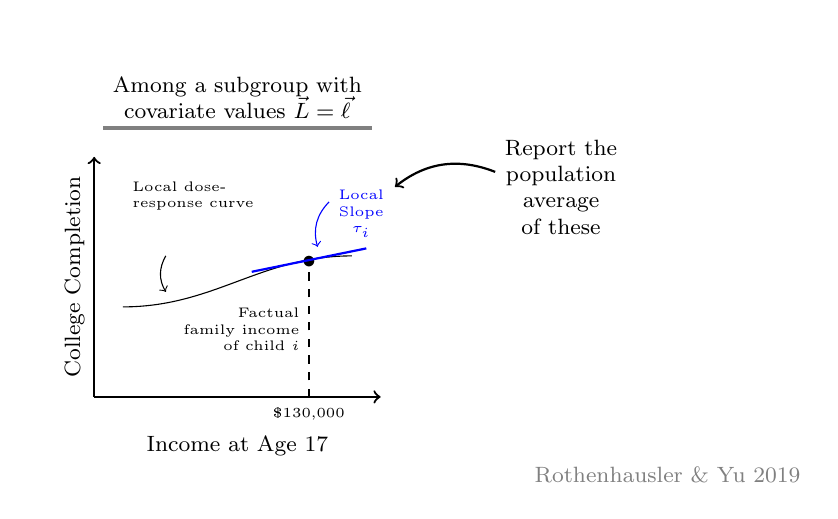
\begin{tikzpicture}[x = .3\textwidth, y = 1.5in]
    % Axes
    \node at (-.2,1.2) {};
    \node<2->[anchor = north, align = center, font = \footnotesize] (among) at (.5,1.1) {Among a subgroup with\\covariate values $\vec{L} = \vec\ell$};
    \draw<2->[line width = 1.2pt, line cap = rounded, gray] (among.south west) -- (among.south east);
    \draw<2->[->, thick] (0,0) -- (1,0);
    \draw<2->[->, thick] (0,0) -- (0,.8);
    %\node<2->[anchor = south, rotate = 90, font = \footnotesize, align = center] at (0,.5) {$\P\big(Y(a) = 1\mid \vec{L} = \vec\ell_i\big)$};
    \node<2->[anchor = south, rotate = 90, align = center, font = \footnotesize] at (0,.4) {College Completion};
    \node<2->[anchor = north, font = \footnotesize, align = center] at (.5,-.1) {Income at Age 17};
    \node<2->[anchor = north west, font = \tiny, align = left] at (.1,.75) {Local dose-\\response curve};
    \draw<2->[->] (.25, .47) to[bend right] (.25,.35);
    \draw<2-> (.1,.3) to[out = 0, in = 180] (.9,.47);
    \node<3->[anchor = east, font = \tiny, align = right] at (.75,.225) {Factual\\family income\\of child $i$};
    \draw<3->[dashed] (.75,0) -- (.75,.45);
    \node<3->[anchor = center] at (.75, .45) {$\bullet$};
    \node<3->[anchor = north, font = \tiny] at (.75,0) {\$130,000};
    % Local slope
    \draw<4->[thick, blue] (.55,.417) -- (.95,.495);
    \node<4->[anchor = south west, align = center, font = \tiny, blue] at (.82, .5) {Local\\Slope\\$\tau_i$};
    \draw<4->[->, blue] (.82,.65) to[bend right] (.78,.5);
    \node<2->[gray, font = \footnotesize, anchor = north east] (cite) at (2.5,-.2) {Rothenhausler \& Yu 2019};
   % \node<5>[font = \footnotesize, anchor = south east, align = center, gray] at (cite.north east) {``Incremental causal effects''};
   \node<5->[font = \footnotesize, anchor = west, align = center] at (1.4,.7) {Report the\\population\\average\\of these};
   \draw<5->[->, thick] (1.4,.75) to[bend right] (1.05,.7);
    \end{tikzpicture}}
\end{frame}

\begin{frame}{Example from a current working paper}

\pause
Locally linear estimation within coarsened subgroups\footnote{This estimation idea comes from: Friedberg, R., Tibshirani, J., Athey, S., \& Wager, S. (2020). \bref{https://doi.org/10.1080/10618600.2020.1831930}{Local linear forests}. Journal of Computational and Graphical Statistics, 30(2), 503-517.}
\vskip .1in
\pause
\begin{enumerate}
\item Learn a random forest
\begin{itemize}
\item Predict college completion
\item Predictors include covariates $\vec{L}$ and treatment $A$
\end{itemize} \pause
\item Each leaf is a coarsened subgroup of $\{\vec{L},A\}$ \pause
\item Within each leaf, estimate OLS with $\{\vec{L},A\}$ as predictors \pause
\item Coefficient on the treatment $\approx$ incremental causal effect
\end{enumerate}

\end{frame}

\begin{frame}

\includegraphics[width = \textwidth]{figures/forest_hist}

\end{frame}

\begin{frame}

\begin{tikzpicture}[x = \textwidth, y = .9\textheight]
\node at (0,0) {};
\node at (1,1) {};
\node[anchor = north, font = \large] at (.65,1) {Describing the covariates of those with};
\node[anchor = north] (small) at (.45,.9) {Small Effects};
\node[anchor = north] (big) at (.85,.9) {Big Effects};
\draw[line cap = rounded, line width = 1.2pt] (small.south west) -- (small.south east);
\draw[line cap = rounded, line width = 1.2pt] (big.south west) -- (big.south east);
%\node[anchor = north west] at (0,.8) {Middle 50\% of conditional average treatment effects};
\node[anchor = north, align = center, font = \footnotesize, gray] at (.45,.83) {-0.1\% to 0.3\%\\increase in P(College)\\per \$10,000 income boost};
\node[anchor = north, align = center, font = \footnotesize, gray] at (.85,.83) {0.6\% to 0.9\%\\increase in P(College)\\per \$10,000 income boost};
\node<2->[anchor = north west] at (0,.6) {\% Black};
\node<5->[anchor = north west] at (0,.5) {\% Hispanic};
\node<7->[anchor = north west, align = left] at (0,.4) {\% Father Absent};
\node<9->[anchor = north west, align = left] at (0,.3) {\% Neither Parent\\Finished College};
\node<11->[anchor = north west, align = left] at (0,.15) {Median\\Income};
\node<3->[anchor = north] at (.45,.6) {19\%};
\node<4->[anchor = north] at (.83,.6) {34\%};
\node<5->[anchor = north] at (.45,.5) {18\%};
\node<6->[anchor = north] at (.83,.5) {25\%};
\node<7->[anchor = north] at (.45,.4) {21\%};
\node<8->[anchor = north] at (.83,.4) {50\%};
\node<9->[anchor = north] at (.45,.3) {74\%};
\node<10->[anchor = north] at (.83,.3) {90\%};
\node<11->[anchor = north] at (.45,.15) {\$77,751};
\node<12->[anchor = north] at (.83,.15) {\$31,433};
\end{tikzpicture}

\end{frame}

\section{Discussion}

\begin{frame}{Continuous treatments: Concluding thoughts}

\begin{tikzpicture}[x = \textwidth, y = \textheight]
\node at (0,0) {};
\node at (1,1.05) {};
\node[anchor = north west] at (0,1) {There exists a common strategy:};
\node<2->[anchor = north] at (.5,.9) {$\begin{aligned}\text{Outcome} = \beta_0 + \beta_1\times\text{Income} &+ \beta_2\times\text{(Confounder 1)} \\&+ \beta_3\times\text{(Confounder 2)} \\&+ \hdots + \epsilon\end{aligned}$};
\node<3->[anchor = north, gray, font = {\footnotesize\bf}, align = center] at (.25,.8) {``effect''\\of\\income};
\draw<3->[->, thick, gray] (.32,.75) to[bend right] (.37,.82);
\node<4->[anchor = north west] at (0,.6) {But the effect actually};
\node<4->[anchor = north west] at (0,.52) {--- varies across people};
\node<5->[anchor = north west] at (0,.45) {--- varies across income values};
\node<4->[anchor = north west] at (.6,.52) {\bblue{heterogeneity}};
\node<5->[anchor = north west] at (.6,.45) {\bblue{nonlinearity}};
\node<6->[anchor = north, align = left] at (.5,.3) {Nonlinear and heterogeneous patterns\\offer opportunities for new discoveries};
\end{tikzpicture}

\end{frame}

\goalsframe

\begin{frame}{Let me know what you are thinking}

\begin{huge} \bref{https://tinyurl.com/CausalQuestions}{tinyurl.com/CausalQuestions} \end{huge}
\vskip .7in

Office hours TTh 11am-12pm and at \bref{https://calendly.com/ianlundberg/office-hours}{calendly.com/ianlundberg/office-hours}\\Come say hi!

\end{frame}

\begin{frame}{If time allows: Discuss}

How would you define the estimand?\\Pick one or invent your own example.
\begin{enumerate}
\item More time exercising causes lower blood pressure.
\item More time sleeping improves focus in class.
\item Reading more pages per day promotes vocabulary development.
\item Smoking more cigarettes causes higher risk of lung cancer.
\end{enumerate}
Things to consider:
\begin{itemize}
\item What treatment values are compared?
\item Over whom will you average those counterfactual outcomes?
\item Are there dangers of extrapolation? How would you mitigate them?
\end{itemize}

\end{frame}

\end{document}

